\chapter{Abstract Framework for DNN Models}

\section{An abstract framework for ANN}
\subsection{Problem: function interpolation}
What we want to do is to approximate a function $f^*: V \to U$, with some given data $\{X^i, Y^i\}_{i=1}^N$. {\bf{But the fact is that, we know only few things about $f^*$!}} If we can know more things about $f^*$, we can design some better model for interpolation such as: 
\begin{itemize}
\item FEM: $f^*$ is a solution of elliptic PDE,
\item Spectral method: $f^*$ has sufficient high smoothness,
\item Deep learning: $f^*$ is produced by the human neural network. 
\item $\cdots$
\end{itemize}
A general idea is to construct a parameters depended function family such $f(W; x)$, where $W \in \mathcal{W}$, so we can have the next simple problem:
\begin{problem}
Find the parameter $\theta^{*}$ such that:
\begin{equation}
\theta^* = \mathop{\arg\min}_{\theta \in \Theta} \sum_{i}^N L(f(\theta;X^i) , Y^i).
\end{equation}
Here $L(\cdot, \cdot)$ is a general metric to define the difference between the real function value $Y^i$ and the predicted out put $f(\theta;X^i)$, a simple example is $ L(f(\theta;X^i) , Y^i) = \|f(\theta;X^i) - Y^i\|^2_{U}$. 
\end{problem}
Then we could choose $f(\theta^*; x)$ as the interpolation of $f$ by given data $\{X^i, Y^i\}_{i=1}^N$.

So, all problem reduced to how to construct a suitable function family $f(W;x): V \to U$. In my opinion, different kinds of machine learning models mean different function families. For example, linear regression means that: 
\begin{equation}
f(\theta; x) = w x + b, \quad \theta = \{w, b \},
\end{equation}
where
\begin{equation}
w \in L(V, U) \quad \text{and} \quad b \in U .
\end{equation}


\subsection{Function family with abstract auxiliary space}
So, now we want to explain the deep learning model based on the idea of function family. The model for deep learning is a little different from the traditional models. The main idea is to imitate the human neural network structure that is the composition of many neurons because $f$ is the reaction of humans for the "input" from real world. But in fact we don't know what real human neural network connection is, so we use a simple idea that those neurons have the hierachical structure. (I will show in the latter, it seems that adding the shortcut connection into those pure hireachical structure will be better.)

From the discussion above, We can take the fully connected feedforward neural network as the composition of affine map and nonlinear map in just some abstract linear space. It means that we construct a nonlinear function from $V$ to $U$ with the auxiliary space $V_i$ with $i = 1:J$ such that we have those next functions:
\begin{equation}\label{equ:affinemap}
A_i: V_{i-1} \to V_i  \quad \text{with} \quad A_i(x) = W_i (x)  + \theta_i  \quad \text{with} \quad W_i \in L(V_{i-1}, V_i) ~~ \theta_i \in V_i.
\end{equation}
and
\begin{equation}
g_i: V_i \to V_i \quad \text{is a general nonlinear function}
\end{equation}
where $i = 0:J$ with $V_0 = V$ and $V_J = U$. 

$$
A_i=(W_i, \theta_i).
$$

So the abstract nonlinear iterative form for $f$ is like:
\begin{equation}\label{equ:abstractNN1}
f = f_{out}\circ f_J,
\end{equation}
with
\begin{equation}\label{equ:abstractNN2}
f_j = g_j(A_j(f_{j-1})), \quad j = 1:J,
\end{equation}
and
\begin{equation}\label{equ:abstractNN3}
f_0 = f_{in}(x), \quad x \in V.
\end{equation}
Here in most cases, $f_0(x)=x$.  But sometimes we can also view $f_0$ as 
denoising process?

We note that
$$
f_j: V\times {\cal W}^j\mapsto V_j. 
$$
and 
$$
f_j(x,{\mathbf A}_j)
$$
where 
$$
{\mathbf A}_j=(A_1,\ldots A_j)=({\mathbf A}_{j-1},A_j).
$$

Notice that
$$
f_0=f_{\rm in}: V=V_0\mapsto V
$$
which is pre-process, and
$$
f_{J+1}=f_{\rm out}: U=V_{J}\mapsto U
$$
which is a post-process.

Generally speaking, if we fix those auxiliary space $V_i$, $g_i$, $f_{in}$ and $f_{out}$, then $f$ only depends on those affine map $A_i \in A(V_{i-1}, A_{i})$ defined in \ref{equ:affinemap}.  So in the abstract form,
\begin{equation}
{\cal W}^j = \Pi_{i=1}^j A(V_{i-1}, V_i).
\end{equation}
\begin{equation}
\mathcal{W} = \Pi_{i=1}^J A(V_{i-1}, V_i).
\end{equation}

\subsection{Loss functions and optimization problems}
Forget about "BP", we first express our problem as:
\begin{problem}Fix $V_i$, $g_i$, $f_{in}$ and $f_{out}$, then the optimization problem is:
\begin{equation}
\mathop{\arg\min}_{{\mathbf A}\in {\cal W}} \sum_{j=1}^N \| f(X^j, {\mathbf A}) - Y^j \|^2_{U}
\end{equation}
\end{problem}

We need to discuss other possible loss functions ....


\section{ANN: a fully connected model}
Once we use general vector space like $\mathbb{R}^n$, $\mathbb{R}^{n_i}$ and $\mathbb{R}^c$ to represent $V$, $V_i$ and $U$. So the affine map from $V_{i-1}$ to $V_i$ can be represented as: 
\begin{equation}
A_i(x) = W_i x + \theta_i, \quad \text{with} \quad W_i \in \mathbb{R}^{n_i \times n_{i-1}} \quad \theta_i \in \mathbb{R}^{n_i}.
\end{equation}
And if the nonlinear map $g_i$ is a little special like:
\begin{equation}
g_i(x_1, \cdots, x_{n_i}) = (g(x_1), \cdots, g(x_{n_i}))^T, \quad \forall i = 1:J,
\end{equation}
where $g$ is a certain nonlinear function form $\mathbb{R}$ to $\mathbb{R}$. Some general choose for $g$ can be: Sigmiod, ReLU and etc.

So the vector representation of the \ref{equ:abstractNN1} to \ref{equ:abstractNN3} is the ANN model exactly. And $J$ is the number of hidden layers and $dim(V_i)$ is the neural numbers for the hidden layer $i$. 

The model will be expressed like:
\begin{equation}\label{equ:repNN1}
f(W;x) = f_{out}\circ f_J,
\end{equation}
with
\begin{equation}\label{equ:repNN2}
f_j = g_j(W_jf_{j-1} + \theta_j), \quad j = 1:J,
\end{equation}
and
\begin{equation}\label{equ:repNN3}
f_0 = f_{in}(x), \quad x \in V.
\end{equation}
So if we fix those auxiliary space by $n_i$, $g_i$, $f_{in}$ and $f_{out}$, all parameters are:
\begin{align}
\mathcal{W} &= \{ (W_i, \theta_i) ~ :  ~ W_i \in \mathbb{R}^{n_{i} \times n_{i-1}} ~ ~\theta_i \in \mathbb{R}^{n_i}, i = 1:J \}, \\
&= \Pi_{i=1}^J ( \mathbb{R}^{n_{i} \times n_{i-1}} \times  \mathbb{R}^{n_i}).
\end{align}


\section{Classification problems}
Now we will state some observation about the classification problems. First is about what kinds of set can be split by linear model(neural network without hidden layers).
\begin{definition}(linear separate)\label{assum:linsep}
Assume that $\{A_i\}_{i=1}^c \subset \mathbb{R}^n$ can be separated by hyperplane by $\{H_i\}_{i=1}^c$ i.e for every $A_i$ there exists $H_i$ such $H_i$ will separate $A_i$ and $\{A_1, \cdots, A_{i-1}, A_{i+1}, \cdots, A_c\}$.
\end{definition}
\begin{lemma}
If the different finite sets $\{A_i\}_{i=1}^c \subset \mathbb{R}^n$ satisfy the assumption \ref{assum:linsep}, then there exists a simple neural network such that 
\begin{equation}
f(x_i) = e_i \quad \forall x_i \in A_i ~~ i= 1:c.
\end{equation}
\end{lemma}
\begin{proof}We can just choose 
\begin{equation}
f(x; \{W,b\})  = H(Wx + b)
\end{equation}
with $W_i$ and $b_i$ define the hyperplane $H_i$ and $H$ is the Heaviside function. Then this $f$ is what we want. So this is a simple neural network without hidden layers.
\end{proof}

%\begin{theorem}[Kernel function]For different finite set $\{A_i\}_{i=1}^c$in $\mathbb{R}^n$(may we need some other conditions), there exists a function $g: \mathbb{R}^n \to \mathbb{R}^m$ such that $\{g(A_i)\}_{i=1}^c$ will satisfy the assumption of linear separable \ref{assum:linsep}.
%\end{theorem}
%\begin{proof}Xiaodong or check literature.
%\end{proof}

\begin{definition}[Separabel]
For different finite set $\{A_i\}_{i=1}^c$in $\mathbb{R}^n$, we say they are separable if there exists a kernel function $g \in (C^0({I^n}))^m$ such that $\{g(A_i)\}_{i=1}^c$ will satisfy the assumption of linear separable \ref{assum:linsep}.
\end{definition}

\begin{remark} Here we show some some cases about the mapping $g$. We can construct a partition of $\mathbb{R}^n$ based on $\{A_i\}_{i=1}^c$, and then use partition of unity we get
$\{g_i\}_{i=1}^c$ with 
\begin{equation}
g_{i}(x) = \delta_{ij} \quad \forall i ~~ \text{and}~~  x \in A_j.
\end{equation}
Then we will have:
\begin{align}
g: \mathbb{R}^n &\to \mathbb{R}^c \\
x &\mapsto (g_1, \cdots, g_c).
\end{align}
This means that, if $x\in A_i$ then
\begin{align}
g(x) = e_i \quad \forall i = 1:c.
\end{align}

This means $\{g(A_i)\}_{i=1}^c$ are just $ m = c$ points and can be linearly separated with sparse structure for $W$. Here one can just take $W = I_{m \times c} = I_{c\times c}$ and $b_i = -\frac{1}{2}$.

What's more, we can think about the binary problems $A_0$ and $A_1$, if there is a manifold $\mathcal{M}$ such that $\mathcal{M}$ can separate them.(We can fix the orientation of $\mathcal{M}$, and makes this statement in mathematics.) If 
\begin{align}
\mathcal{M} = \{ x ~ | ~ \phi(x) = 0\},
\end{align}
with $\phi \in C^{\infty}(\mathbb{R}^n)$. So, here you have two ways to choose the mapping,
\begin{itemize}
\item Just choose $g = \phi$, then this satisfy this condition of the continuity of $\phi$.
\item If $\phi = \sum_{i=1}^m w_i \phi_i + b = 0$, so we can take $g = (\phi_1, \cdots, \phi_m)$, and the separation hyperplane is:
\begin{align}
\sum_{i=1}^m w_i y_i + b = 0,
\end{align}
in $\mathbb{R}^m$.
\end{itemize}

{\bf But, how to extend this binary problems into multi-classification problems in this way seems to 
non-trival.}

\end{remark}


\begin{theorem}
For different finite set $\{A_i\}_{i=1}^c$in $\mathbb{R}^n$ satisfy the separable condition, then there exists a DNN model with one hidden layer such that 
\begin{equation}
f_\theta(x_i) = e_i \quad \forall x_i \in A_i \quad i = 1:c,
\end{equation}
with 
\begin{align}
f_{\theta}(x) = H(W_2\sigma(W_1x + b_1) + b_2).
\end{align}
What's more, we can set $W_2 \in \mathbb{R}^{c \times N}$ with 
\begin{equation}
W_2 = W \cdot K,
\end{equation}
such that $W \in \mathbb{R}^{c \times m}$ and $K \in \mathbb{R}^{m \times N}$.
\end{theorem}
\begin{proof}
First, there exists a $g$ and $H(Wx + b)$ such that
\begin{align}
\tilde{f}_{\theta}(x_i) = H(W\tilde{g}(x_i) + b) = e_i \quad \forall x_i \in A_i \quad i = 1:c.
\end{align}

Then by the continuous and properties of Heaviside function, there exists $\epsilon > 0$ such that so for any $g \in  (C^0({I^n}))^m$ with 
\begin{align}
\|g - \tilde{g}\|_{L^{\infty}} \le \epsilon.
\end{align}
We will have
\begin{align}
f_{\theta}(x_i) = H(Wg(x_i) + b) = e_i \quad \forall x_i \in A_i \quad i = 1:c.
\end{align}

Because of the universal approximation theory for artificial neural network, i.e. there exists a network like 
\begin{align}
g(x) = K\sigma(W_1 x + b_1) + \alpha,
\end{align}
with 
\begin{align}
K = \mathrm{diag}\{K_1, \cdots, K_m\}, \quad K_i \in \mathbb{R}^{1\times n_i}  \quad N = \sum_{i=1}^m n_i,
\end{align}
such that
\begin{align}
\|g - \tilde{g}\|_{L^{\infty}} \le \epsilon.
\end{align}

So 
\begin{align}
f_{\theta}(x_i) = H(W_2\sigma(W_1x_i + b_1) + b_2) = e_i \quad \forall x_i \in A_i \quad i = 1:c,
\end{align}
and 
\begin{equation}
W_2 = W \cdot K,
\end{equation}
with $W \in \mathbb{R}^{c \times m}$ and $K \in \mathbb{R}^{m \times N}$.

\end{proof}


\section{CNN model under this framework}
\subsection{Simple convolution introduction(without multichannel)}
There is a kind of special linear map from some general finite dimension tensor space to another is called ``convolution".  Generally, we have a tensor like $X \in \mathbb{R}^{n \times m}$ and a small kernel such as $K \in \mathbb{R}^{k\times k}$, then we have:
\begin{definition}[Original Convolution with stride 1 for CNN]
\begin{equation}\label{equ:conv}
(X\ast K)_{i,j} = \sum_{s, t = 1}^k X_{i-1 + s, j-1 + t} K_{s,t}.
\end{equation}
It's easy to see that $(X\ast K) \in \mathbb{R}^{(n-k + 1) \times (m-k + 1)}$.
\end{definition}
If we use stride $p$, we have:
\begin{definition}[Original Convolution with stride $p$ for CNN]
\begin{equation}\label{equ:convstride}
(X\ast_{p} K)_{i,j} = \sum_{s, t = 1}^k X_{(i-1)p + s, (j-1)p + t} K_{s,t}.
\end{equation}
So, we have 
$
(X\ast_p K) \in \mathbb{R}^{((n-k)/p + 1) \times ((m-k)/p+1)}.
$
\end{definition}
This stride properties in some application is be used as pooling(subsampling, coarsening).  

Here we can define a special pooling operator as $S^p$ which likes the $C/F$ split for choosing coarse point:
\begin{equation}
S^p(X)_{i,j} = X_{(i-1)p + 1, (j-1)p + 1},
\end{equation}
then we have:
\begin{equation}\label{equ:stride}
X \ast_p K = S^p(X\ast K),
\end{equation}
with the $\ast$ and $\ast_p$ defined by \ref{equ:conv} and \ref{equ:convstride}
\begin{proof}
\begin{align}
S^p(X \ast K)_{i,j} &= (X \ast K)_{(i-1)p+1, (j-1)p + 1}  \\
&= \sum_{s,t = 1}^k X_{(i-1)p + 1 -1 +s, (j-1)p +1 -1 +t}K_{s,t}  \\
&= (X \ast_p K)_{i,j}.
\end{align}
\end{proof}

\subsubsection{Convolution(without changing size)}
For many case kernel size is some small odd numbers such as 1, 3, 5... So we ca have those next definition for convolution:
\begin{definition}[Convolution with Padding]

We write $K\in \mathbb R^{2k+1, 2k+1}$, we then write
\begin{equation}\label{ConvPadding}
(X \hat{\ast} K)_{i,j} := (\rm{P}^k(X) \ast K)_{i,j} = \sum_{s, t = -k}^k X_{i + s, j + t} K_{s,t},
\end{equation}
with $\rm{P}^k$ means Padding. 
\end{definition}
Here we see that, to make this definition well-defined, we have $X\ast K \in \mathbb{R}^{n-2k, m-2k}$, because if the index of $X$ start from $1$ to $n(m)$, then $X \ast K$ from $k+1$ to $n(m) - k$. To make the convolution don't change size, we can use Padding strategy like in image process. 
%In fact, if the resolution is very high, which means the measure of the boundary of the image is close to 0, so in traditional image process, this strategy hasn't been studied very well. There are basic three strategy:
\begin{description}
\item[Zero Padding] The simplest and most common used strategy is zero padding with:
\begin{equation}
\rm{P}^k_0: \mathbb{R}^{n \times m} \to \mathbb{R}^{n+2k \times m+2k}
\end{equation}
with 
\begin{equation}
\rm{P}_0^k(X)_{i,j} = \begin{cases}
0 &i(j)=-k+1:0 ~~\text{and}~~ i(j) = n(m)+1:n(m)+k \\
X_{i,j} &i(j) = 1:n(m) 
\end{cases}
\end{equation}
\item[Reflection Padding] This strategy is defined by:
\begin{equation}
\rm{P}^k_r: \mathbb{R}^{n \times m} \to \mathbb{R}^{n+2k \times m+2k}
\end{equation}
with 
\begin{equation}
\rm{P}_r^k(X)_{i,j} = \begin{cases}
X_{1-i, 1-j} &i(j)=-k+1:0 ~~\text{and}~~ i(j) = n(m)+1:n(m)+k \\
X_{i,j} &i(j) = 1:n(m) \\
0 &\text{others} 
\end{cases}
\end{equation}
\item[Shift Padding] This strategy is defined by:
\begin{equation}
\rm{P}^k_s: \mathbb{R}^{n \times m} \to \mathbb{R}^{n+2k \times m+2k}
\end{equation}
with 
\begin{equation}
\rm{P}_s^k(X)_{i,j} = \begin{cases}
X_{k-i, k-j} &i(j)=-k+1:0 ~~\text{and}~~ i(j) = n(m)+1:n(m)+k \\
X_{i,j} &i(j) = 1:n(m) \\
0 &\text{others} 
\end{cases}
\end{equation}
\end{description}

So we can have:
\begin{equation}
\rm{dim}(X\hat{\ast}K) = \rm{dim}(\rm{P}^k(X) \ast K) = \rm{dim}(X),
\end{equation}
and the $i,j$ index is consistent for both side of the above equation where $\rm{P}^k = \rm{P}_0^k, \rm{P}_{r}^k$ or $\rm{P}_s^k$.


\begin{remark}We note all the later convolution as the \eqref{ConvPadding} for consistent.

\end{remark}

\subsection{Convolution with multichannel}
\subsubsection{Traditional convolution for multichannel case}
Here in real data, we have some special data like colour image $X \in \mathbb{R}^{n \times m \times3}$. Here this image is a 2D graph, with $3$ means the $RGB$ channels. So, we cannot just think $X$ as a general $3$-order tensor. We may just use this as an example, $X \in \mathbb{R}^{n\times m \times c}$, we say that $n \times m$ is the essential dimension and $c$ is the channel dimension for $X$. If we want to do convolution for $X$, here we cannot just use $K \in \mathbb{R}^{k\times k}$ because of multichannel. A simple idea is to use also different $c$ kernels and collect them together as $K \in \mathbb{R}^{k\times k \times c}$, and then we can do the general convolution for signal channel separately. This means that 
\begin{equation}
(X\ast_{p} K)_{i,j,l} = \sum_{s, t = 1}^k X_{(i-1)p + s, (j-1)p + t,l} K_{s,t,l},
\end{equation}
and $(X\ast_p K) \in \mathbb{R}^{((n-k)/p + 1)\times ((m-k)/p+1) \times c}$. But we need to recall that, even for $X \in \mathbb{R}^{n\times m \times c}$ it is in fact only stand for just one 2D image(with multi-channel). So if we talk about features in AI, $(X\ast_p K) \in \mathbb{R}^{((n-k)/p + 1)\times ((m-k)/p+1) \times c}$ should be reduced to the essential dimension, one simple way is just to add all the channels value together w.r.t essential dimension(this is equal to added with weights because we can reduce those DoF into the previous $c$ kernels.):
\begin{equation}
(X \hat{\ast}_p K)_{i,j} = \sum_{l=1}^{c} \sum_{s, t = 1}^k X_{(i-1)p + s, (j-1)p + t,l} K_{s,t,l},
\end{equation}
then we have
\begin{equation}
(X \hat{\ast}_p K) \in \mathbb{R}^{((n-k)/p + 1) \times ((m-k)/p+1)} \quad \text{with} \quad K \in \mathbb{R}^{n \times m \times c}.
\end{equation}
So, for a given real data with $c$ channels like $X \in  \mathbb{R}^{n\times m \times c}$ if we use kernel $K \in \mathbb{R}^{k\times k \times c}$ we can only get a signal channel output. To get multichannel form $X$, we just need to use $d$ kernels $K \in \mathbb{R}^{k\times k \times c}$, or we say $K \in \mathbb{R}^{k\times k \times c \times b}$, then we have:
\begin{equation}\label{6.6}
(X \hat{\ast}_p K)_{i,j,g} = \sum_{l=1}^{c} \sum_{s, t = 1}^k X_{(i-1)p + s, (j-1)p + t,l} K_{s,t,l,g},
\end{equation}
with 
\begin{equation}
(X \hat{\ast}_p K) \in \mathbb{R}^{((n-k)/p + 1) \times ((m-k)/p+1) \times b} \quad \text{with} \quad K \in \mathbb{R}^{n \times m \times c \times b}.
\end{equation}

In the next section, we set that all tensor is with
multichannel(signal channel is a special case, and we note it as $X
\in \mathbb{R}^{n \times m \times 1}$), and we just use $\ast_p$ no
longer $\hat{\ast}_p$.

\subsubsection{New version}
Here we consider our data like $T = (T_1, T_2, T_3)$ with $T_i \in \mathbb{R}^{n\times n}$.

Prof. Xu's idea is to say that, we need to keep the original ``channel" parallel i.e we just need three kernels like 
\begin{align}
K_0 = \begin{pmatrix}
K^1 \\ K^2 \\ K^3
\end{pmatrix}.
\end{align} So we get:
\begin{equation}
T \to T\tilde{\ast} K_0 = (T_1 \ast K^1, T_2\ast K^2, T_3 \ast T^3),
\end{equation}
and then we apply the active function $a$ to $(T_1 \ast K^1, T_2\ast K^2, T_3 \ast T^3)$ element by element. And then use 
\begin{align}
T^{new} = (a(T_1 \ast K^1), a(T_2\ast K^2), a(T_3 \ast T^3))
\end{align} as the next input for the CNN network.
 
Now we want to show that the traditional method with more kernels can reproduce the $T^{new}$ in Prof. Xu's case.

Here we set we have some more kernels like 
\begin{align}
K = 
\begin{pmatrix}
K_1^1 & \cdots & K_1^N \\
K_2^1 & \cdots & K_2^N \\
K_3^1 & \cdots & K_3^N 
\end{pmatrix},
\end{align} with $K_i^j \in \mathbb{R}^{3\times3}$.

What we have at most are:
\begin{equation}
\tilde{T} = T\tilde{\ast} K =  \begin{pmatrix}
T_1 \ast K_1^1 & \cdots & T_1\ast K_1^N \\
T_2 \ast K_2^1 & \cdots & T_2\ast K_2^N \\
T_3 \ast K_3^1 & \cdots & T_3\ast K_3^N 
\end{pmatrix}
\end{equation}

{\bf Here in fact we can have a simple question: why we don't just put $a(\tilde{T})$ as the next input for the next layer of CNN? Maybe this dimension is to large?}

Traditional method for convolution with channel is to say we need to compress the original ``channel" dimension by take 
\begin{equation}
\tilde{T}  \to ( \sum_{j=1:3} T_j\ast K_{j}^1, \cdots, \sum_{j=1:3} T_j\ast K_{j}^N),
\end{equation} 
and then apply the active function $a$ getting:
\begin{equation}
(a( \sum_{j=1:3} T_j\ast K_{j}^1), \cdots, a(\sum_{j=1:3} T_j\ast K_{j}^N)).
\end{equation}

So we can see that, if we take $ N = 3$ then we can reproduce the 
$T^{new} = (a(T_1 \ast K^1), a(T_2\ast K^2), a(T_3 \ast T^3))$ from $(a( \sum_{j=1:3} T_j\ast K_{j}^1), \cdots, a(\sum_{j=1:3} T_j\ast K_{j}^N))$ by just take
\begin{align}
K^i = \sum_{j=1:3} K_j^i, \quad \forall i = 1:3.
\end{align}

\begin{remark}
Here we can take Prof. Xu's idea and the traditional convolution as consistent by means that because the dimension for $a(\tilde{T})$ is too large({\bf In fact, we like redundancy some times, why we just use this directly?}), we need some ways to compress $\tilde{T}$ first and then apply active function $a$. The simplest next two ways is:
\begin{itemize}
\item Compress(sum) $\tilde{T}$ in row. This leads to Prof. Xu's idea keeping the ``channel" number as 3.
\item Compress(sum) $\tilde{T}$ in column. This leads to traditional idea changing the ``channel" into $N$.
\end{itemize}

{\bf Another questions is how to compress this $\tilde{T}$ ``better"?  What dose better means?}
 
\end{remark}
 
\subsection{Convolution with vectorization and matrix tensor product}
\subsubsection{Vectorization and matrix tensor product}
First, we can define the next vectorization operator:
\begin{equation}
\rm{Vec}: \mathbb{R}^{n \times m} \to \mathbb{R}^{nm}
\end{equation}
with 
\begin{equation}
(\rm{Vec}(X))_{(i-1)m + j} = X_{ij}.
\end{equation}

In this notation, for a discrete $u_{i,j}$ with $ i, j = 1:n$, we can have the next 5-points difference scheme with:
\begin{equation}
\rm{Vec}(\Delta_h u) = M_5 \rm{Vec}(u),
\end{equation}
with 
\begin{equation}
M_5 = T\otimes I_{n} + I_{n} \otimes T,
\end{equation}
where $T$ is the $1-D$ mid-point difference matrix like: 
\begin{equation}
T = \rm{tridiag}(-1,2,-1) \in \mathbb{R}^{n \times n}
\end{equation}

\subsubsection{5-points difference as a special convolution}
For general convolution definition, the convolution operator will reduce the dimension for the input data. Here we begin with $1-D$ case, like $K \in \mathbb{R}^{3}$, then for a vector $X \in \mathbb{R}^n$, we do the general convolution with stride 1, then we have 
\begin{equation}
X \ast K \in \mathbb{R}^{n-2},
\end{equation}
and if we take $K = (-1, 2, -1)$, then
\begin{equation}
X \ast K = \Delta_h X_{2:n-1},
\end{equation}
with boundary condition $X_{\rm{left}} = X_1$ and $X_{\rm{right}} = X_n$.  

To preserve the dimension, we can use the ``Padding" operator for $1-D$:
\begin{equation}
\rm{Pad}(X) = (0, X, 0),
\end{equation}
there are similar definition for $n-D$ tensor. 

Then we have:
\begin{equation}
\rm{Pad}(X) \ast K = \Delta_h X = T X.
\end{equation}

So for $2-D$ case $u \in \mathbb{R}^{n \times n}$, and 
\begin{equation}
K = 
\begin{pmatrix}
0 & -1 & 0 \\
-1 & 4 & -1 \\
0 & -1 & 0 
\end{pmatrix}
\end{equation}
then we have: 
\begin{equation}
\rm{Vec}(\rm{Pad}(u) \ast K ) = \rm{Vec}(\Delta_h u) = M_5 \rm{Vec}(u).
\end{equation}


\subsection{Convolution explained by liner map with special structure}
CNN can also be recovered by the abstract form above with the represent of $V_i$ to be general tensor space. For example, $V_{i-1} = \mathbb{R}^{n \times m}$ and $V_i = \mathbb{R}^{l}$, then we can just set 
\begin{equation}
A_i(X) = WX + \theta \in V_i,
\end{equation}
where
\begin{equation}
(WX)_{g} = \sum_{s,t=1}^{n,m}W_{s,t,g}X_{s,t}, \quad W \in \mathbb{R}^{l \times n \times m}
\end{equation}

Just as what we see above, the dimension of $V_i$ can not be arbitrary, it is defined by the kernel and stride size and the numbers of the kernel. 

An example for this is like that, $X \in V_{i-1}$ is a signal channel 2D tensor, and we choose just one kernel $K \in \mathbb{R}^{k\times k}$ with stride p, which means that $V_i = \mathbb{R}^{(n-k)/p + 1)\times ((m-k)/p+1)}$.  Then the $W \in \mathbb{R}^{((n-k)/p + 1)\times ((m-k)/p+1) \times n \times m}$ should be like: 
{\small{
\begin{equation}
W_{i,j, s,t} = \begin{cases}
K_{s-(i-1)p,t-(j-1)p} ~ &\text{if} ~ s \in (i-1)p+1:(i-1)p+k ~ \& ~ t \in (j-1)p+1:(j-1)p+k \\
&0.
\end{cases}
\end{equation}
}}
Now if we consider $X \in V_{i-1} = \mathbb{R}^{n \times m \times c }$ with $c$ channels and we choose kernel as $K \in \mathbb{R}^{k\times k \times c \times b}$ and use convolution with stride p, which means $V_{i} = \mathbb{R}^{((n-k)/p + 1)\times ((m-k)/p+1) \times b}$. So we have 
\begin{equation}
W \in L(V_{i-1}, V_i) = \mathbb{R}^{(((n-k)/p + 1)\times ((m-k)/p+1) \times b) \times (n \times m \times c)},
\end{equation}
with 
{\small{
\begin{equation}
W_{i,j,g, s,t,l} = \begin{cases}
K_{s-(i-1)p,t-(j-1)p,l,g} ~ &\text{if} ~ s \in (i-1)p+1:(i-1)p+k ~ \& ~ t \in (j-1)p+1:(j-1)p+k \\
&0.
\end{cases}
\end{equation}
}}
Then we have:
\begin{equation}
WX = X \ast_p K.
\end{equation} 


At last, in the CNN model, the shift vector $\tilde\theta \in V_i$ is also have a special structure with
\begin{equation}
\tilde\theta_{i,j,l} = \theta_l,
\end{equation}
which means $dim(\tilde\theta) = b = $ the number of kernels in $K$. Which means that:
\begin{equation}
dim(W) + dim(\tilde\theta) = dim(K) + dim(\tilde\theta) = k\times k \times c \times b + b \neq dim(L(V_{i-1}, V_i)) + dim(V_i).
\end{equation}

\subsection{Active function}


\subsection{Pooling and convolution with stride}
Just as saying before, if $X \in V_{i-1} = \mathbb{R}^{n \times m \times c }$ with $c$ channels and we choose kernel as $K \in \mathbb{R}^{k\times k \times c \times b}$ and use convolution with stride p, then we have
\begin{equation} 
V_{i} = \mathbb{R}^{((n-k)/p + 1)\times ((m-k)/p+1) \times b},
\end{equation}
which means that the essential dimension of $X$ was almost decreased to $\frac{1}{p}$, which is almost like result of the pooling(subsampling or coarsening) operation. So, in some recent popular CNN models, they often choose the convolution with stride $2$ as the a combination of convolution and pooling layers.

However, we can say that, some general pooling operation is in fact nonlinear operation but convolution with stride $p$ is still a special linear map and this may also change the channel dimensions. So we would like to added the pooling operation as a special kind of restriction, such as $X \in V_{i-1} = \mathbb{R}^{2n \times 2m \times c }$ then 
\begin{equation}
R(X)_{i,j,l} = r(X_{(2i - 1:2i), (2j-1:2j),l}),
\end{equation}
with $r(\bm{x})$ can be:
\begin{itemize}
\item Maxout: $r(\bm{x}) = \max \{x_1, \cdots, x_4\}$,
\item Average: $r(\bm{x}) = \frac{\sum_{i=1}^4 x_i}{4}$,
%\item $L^2$ normal: $r(\bm{x}) = \|x\|$,
\item $\cdots$
\end{itemize}
Here we see that $R: V_i \to \hat{V}_i$ only change the essential dimension for $X$ and apply $r$ separately w.r.t channel dimension. In real application, you can also use the channel-cross pooling strategy which will a little like the convolution with stride.

\subsection{General structure for CNN}
A general CNN model is the composition of convolution, nonlinear map and pooling layers then followed with few ANN layers. 
Now we still assume that data is like $\{X^i, Y^i\}_{i=1}^N$ with $X_i \in V_0$ and $Y_i \in U$. We choose some auxiliary space $V_i$, $\hat{V}_i$ with $i = 1:J$ and $U_i$ with $i = 1:L$. 

We can use just $f_{ANN}(W_A; x)$ to denote the ANN model from $V_J$ to $U$ with auxiliary space $U_i$ with $i = 1:L$.

And the CNN part can be expressed as:
\begin{align}
f_{CNN} &= f_J(W_{CNN};x), \\
f_j &= R_j \circ g(W_i f_{j-1} + \tilde{\theta}_i), \quad j = 1:J \\
f_0 &= x.
\end{align}
\begin{itemize}
\item For many real CNN models, $R_j = \rm{id}$ for many $j \in 1:J$. 
\item This likes a slash cycle with many smooth steps in every level.
\item The reason why they need so many smooth steps is to increase the parameter numbers, so try general cycle might be a interesting method.
\end{itemize}

Ana at last, we get a general CNN model as:
\begin{equation}
f(W;x) = f_{ANN}(W_{ANN}; f(W_{CNN};x)), \quad \text{with} \quad W = \{W_{ANN}, W_{CNN}\}.
\end{equation}



\section{RNN model under this framework}
\subsection{A simple example of RNN}
Here we consider our problem with data like $X^i = (x^{i,(1)}, \cdots, x^{i,(t)}, \cdots, x^{i,(\tau)})$ with $x^{i,(t)} \in V^{(t)} = V$ for all $t = 1:\tau$ and $Y^i = (y^{i,(1)}, \cdots, y^{i,(t)}, \cdots, y^{(i,\tau)})$ with $y^{i,(t)} \in U^{(t)} = U$ for all $t = 1:\tau$. So, we can say that:
\begin{equation}
X \in \bar{V} = \underbrace{V\times V \times\cdots \times V }_{\tau} ~\text{and}~ Y \in \bar{U} =  \underbrace{U\times U \times\cdots \times U }_{\tau}.
\end{equation}
So we can use the similar idea in ANN, by choose auxiliary space $V_i$ and construct:
\begin{equation}
\bar{V}_i = \underbrace{V_i \times V_i \times \cdots \times V_i}_{\tau}, \quad i = 1:J.
\end{equation}

So, we can also talk about the ANN with $\bar{V}_i$ $i = 0:J+1$ like the definition in \ref{equ:abstractNN1} to \ref{equ:abstractNN3}. What's more, if 
\begin{equation}
\bar{W}_i = \text{diag}(W^{(1)}_i, \cdots, W_i^{(\tau)}),
\end{equation}
and $g_i$ is a nonlinear map form $V_i^{(t)}$ to $V_i^{(t)}$. Then the ANN model form $\bar{V}$ to $\bar{U}$ is just $\tau$ separate ANN model form $V$ to $U$. So, a naive idea to change this should be choose $\bar{W}_i$ not be block diagonal matrix. {\bf{But, this is not RNN!}}

Now we show a simple RNN model with:
\begin{align}
f_{1}^{(t)} &= g_1^{(t)}(\theta_1 + W_1f_1^{(t-1)} + U_1x^{(t)}), \\
f_{2}^{(t)} &= \theta_2 + U_2f_{1}^{(t)}, \\
f^{(t)} &= \rm{softmax}(f_2^{(t)}).
\end{align}

Also we can have this kind of RNN network:
\begin{align}
f_{1}^{(t)} &= g_1^{(t)}(\theta_1 + W_1f_2^{(t-1)} + U_1x^{(t)}), \\
f_{2}^{(t)} &= \theta_2 + U_2f_{1}^{(t)}, \\
f^{(t)} &= \rm{softmax}(f_2^{(t)}).
\end{align}

So it seems that, we can have the next definition for RNN:
\begin{equation}\label{equ:abstractRNN1}
f = f_{out}\circ f_J,
\end{equation}
with
\begin{equation}\label{equ:abstractRNN2}
f^{(t)}_j = g_j(\bar{A}_j(f^{(t)}_{j-1}) + \bar{W}_{j}^j f^{(t-1)}_{j}),
\end{equation}
and
\begin{equation}\label{equ:abstractRNN3}
f_0 = f_{in}(x), \quad x \in \bar{V}.
\end{equation}
Here 
\begin{equation}
\bar{W}_j^{j} \in L(\bar{V}_j, \bar{V}_j), \text{is a blocked lower triangular matrix}.
\end{equation}
which is invariant through all timesteps from $t=1$ to $\tau$. \\
This formula seems the symmetric form for the next section about the shortcut connection form.
\subsection{Development of the simple RNN}
Note that $\bar{W}_j^j$ denotes the relation between $V_j^{(t-1)}$ with $V_j^{(t)}$,we suppose that the relation is the same through all the timesteps, which is similar to the model of Markov chain. \\
However, there exists some problems is the $\bar{W}_j^j$ is a simple affine transformation. With the same matrix multiplied by many times, the eigenvalues will explode or decay to zero quickly. That leads to gradient exploding or gradient vanishing, which makes the simple model hard to capture the long-term dependence. Here we introduce the LSTM model to solve the problem. \\
Here we transforms the $\bar{A}_j$ and $\bar{W}_j^J$ into the following form:
\begin{equation}
f^{(t)}_j = g_j (\bar{W}_{j}^j (f^{(t-1)}_{j},f^{(t)}_{j-1})),
\end{equation}
\begin{equation}
\bar{W}_{j}^j (f^{(t-1)}_{j},f^{(t)}_{j-1}) = \sigma_1 \ast s_j^{(t-1)} + \sigma_2 \ast q_j^{(t)}
\end{equation}
where
\begin{align}
s_j^{(t-1)} & = g_j^{-1} f_j^{(t-1)} = \bar{A}_j(f^{(t-1)}_{j-1}) + \bar{W}_{j}^{j} f^{(t-2)}_{j} \\
\sigma_1 & = g_j^{(f)}(\bar{A}_j^{(f)}(f^{(t)}_{j-1}) + \bar{W}_{j}^{j^{(f)}} f^{(t-1)}_{j}) \\
\sigma_2 & = g_j^{(g)}(\bar{A}_j^{(g)}(f^{(t)}_{j-1}) + \bar{W}_{j}^{j^{(g)}} f^{(t-1)}_{j}) \\
q_j^{(t)} & = g_j^{(n)}(\bar{A}_j^{(n)}(f^{(t)}_{j-1}) + \bar{W}_{j}^{j^{(n)}} f^{(t-1)}_{j})
\end{align}
The superscripts f and g denote the 'forget' and 'get' gating, which control which part of $f_j^{(t-1)}$ and $f_{j-1}^{(t)}$ can be transformed into $f_j^{(t)}$.Here $\bar{A}_j^{(f)} $,$\bar{W}_{j}^{j^{(f)}}$,$\bar{A}_j^{(g)}$ and $\bar{W}_{j}^{j^{(g)}}$ are of the same definition in the simple RNN model. That's exactly the LSTM model. \\
Also,the LSTM model can be simplified into the GRU model, which keeps $\sigma_1$ with the same definition, while$\ \sigma_2 = 1 - \sigma_1$.That saves some cost of the computation.


\section{Shortcut connection}
First, we would like to talk about the so called ``shortcut connection" in general neural network. It can be defined more generally by
\begin{equation}
f_j = g_j(A_j(f_{j-1} + \sum_{i=0}^{j-2}\tilde{W}_i^j f_i)) = g_j( \sum_{i=0}^{j-1}W_i^{j}f_i + \theta_j),
\end{equation}
where 
\begin{equation}
W_i^j \in  L(V_i, V_j) \quad \text{and} \quad W_j = W_{j-1}^j. 
\end{equation}
\subsection{ResNet}
The most important structure in ResNet model is the ``shortcut connection'' with 2-shortcusts, i.e:
\begin{align}
&f = f_{out}\circ f_J, \\
&\begin{cases}
f_j = g_j(A_jf_{j-1} + I_jf_{j-2}), \quad &\text{for} ~j~ \text{is odd} \\
f_j = g_j(A_jf_{j-1}), \quad  &\text{for} ~j~ \text{is even},
\end{cases} \\
&f_0 = x.
\end{align}

Here the convolution in ResNet adopt padding with zero such that the essential dimension will not change expect after the pooling layers. So in many case $I_j$ is just identity operator. If the are dimension reduction in essential dimension the $I_j$ is a simple restrict operator which needs to learn and just add zeros for the channel dimension. 

\subsection{Two-grid method}
So, if we use the shortcut connection in a general ANN model, we can recover the simple two-grid scheme to solve $Au = b$ from $u^k$ to $u^{k+1}$ with $u^k \in V = U = \mathbb{R}^n$.

One thing I need to mention again is that, here we just use the network frame to recover the two-grid iterative scheme, all $A_i$ and $g_i$ is defined by ourself, one on need to be learnt. 

Here we set $g_i = id$ for $i = 1:6$.  And $V_i = V$ for $i = 1,4,5,6$ and $V_i = V_c$ for $i = 2,3$, where $V_c$ is the coarse space. $P$ is the interpolation operator form $V_c$ to $V$ and $A_c = P^T A P$, $R$ is the smoother on the fine grid. So we have the next definition of $A_i$: 
\begin{itemize}
\item $f_1 = A_1(f_0) = b - Af_0$,
\item $f_2 = A_2(f_1) = P^T f_1$,
\item $f_3 = A_3(f_2) = A^{-1}_c f_2$,
\item $f_4 = A_4(f_3) = P f_3$,
\item $f_5 = A_5(f_4) + W_1^5 f_1 =f_1 -  Af_4$,
\item $f_6 = A_6(f_5) + W_0^6 f_0 + W_4^6 f_4 = f_0 + f_4 + Rf_5$.
\end{itemize}
Then if we take $f_0 = u_k$ we will have $f_6 = u^{k+1}$ comes from a two-grid step with 
\begin{equation}
u^{k+1} = u^{k} + B(b - A u^k),
\end{equation}
with $Bg$ is defined by
\begin{align}
w &= PA_c^{-1}P^{T}g, \\
Bg &= w + R(g - Aw). 
\end{align}

In this point of view, it seems that adopting the shortcut connection in deep learning seems to make sense. And just as we mentioned before, we don't know what real human neural connections, and deep learning with shortcut connection will more general to approximate the human neural network. What's more, a popular CNN model ResNet used this structure and won the ImageNet classification challenge in 2015.

\section{U-Net and multigrid model in CNN}
Fro traditional CNN model, especially for classification or locallization problem, the general CNN model w.r.t essential dimension like a slash cycle very much, such as AlexNet, VGGNet or ResNet. But for segmentation problem, because of the high dimension of both input and output data, CNN model wasn't very popular for some reasons. Traditional method with image process still is the main methods. But in 2105, [ ] proposed a network to dealt with biology cell image segmentation problem, and win the ISBI challenge for segmentation of neuronal structures in electron microscopic stacks. The U-Net structure of essential dimension likes the V-cycle very much. 

\begin{figure}[!htb]        
	\center{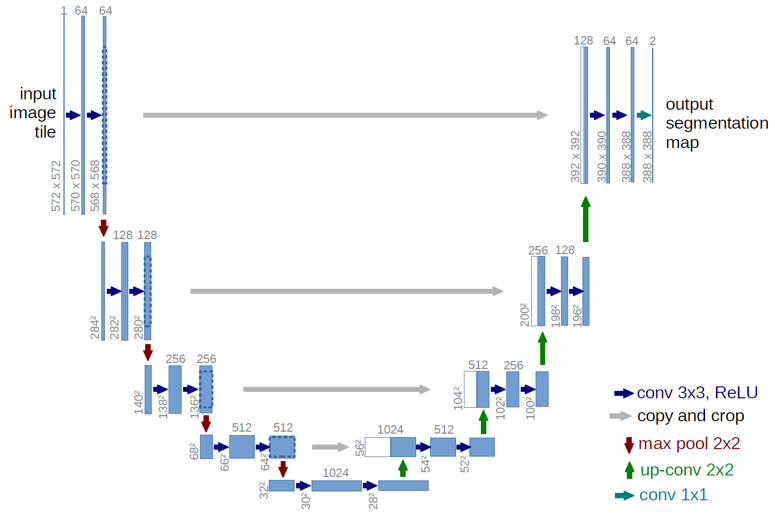
\includegraphics[width=12cm] {UNetAIMedical1.png}}        
	\caption{Architecture for U-Net}      
	\label{U-Net-model}
\end{figure}

\newpage